\begin{frame}
\frametitle{The cone over $\dP6$}

\begin{columns}
\column{0.5\textwidth}

\begin{itemize}
	\item Let $\dP6 \subset \P^6$ be an anticanonically embedded del Pezzo surface of degree $6$. Let $C(\dP6)$ be its affine cone in $\mathbb A^7$.

	\item The equations are 
	$$
\begin{vmatrix}
y & x_1 & x_2 \\
x_4 & y & x_3 \\
x_ 5 & x_6 & y
\end{vmatrix}
\leq 1
	$$

The origin is an isolated singularity.

\end{itemize}


\column{0.5\textwidth}

\begin{itemize}
	\item There are two smoothing components.
	\item They come from perturbations of differents form of writing the equation.
	\item Can also write the equations as:

	\begin{center}
	
	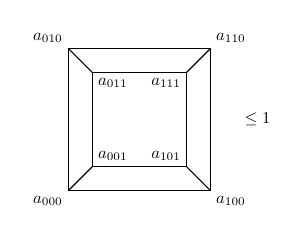
\begin{tikzpicture}[scale=0.6, every node/.style={scale=0.6}]
\draw (0,0) -- (3,0) -- (3,3) -- (0,3) -- cycle;
\draw (0.5,0.5) -- (2.5,0.5) -- (2.5,2.5) -- (0.5,2.5) -- cycle;
\draw (0,0) -- (0.5,0.5);
\draw (3,0) -- (2.5,0.5);
\draw (3,3) -- (2.5,2.5);
\draw (0,3) -- (0.5,2.5);
\node[below left] at (0,0) {$a_{000}$};
\node[below right] at (3,0) {$a_{100}$};
\node[above right] at (3,3) {$a_{110}$};
\node[above left] at (0,3) {$a_{010}$};

\node[above right] at (0.5,0.5) {$a_{001}$};
\node[above left] at (2.5,0.5) {$a_{101}$};
\node[below left] at (2.5,2.5) {$a_{111}$};
\node[below right] at (0.5,2.5) {$a_{011}$};

\node at (4, 1.5) {$\leq 1$};
\end{tikzpicture}
\end{center}
\end{itemize}

\end{columns}
\end{frame}

\begin{frame}
\frametitle{The two smoothing compoments of $\dP6$}
\begin{columns}
\column{0.5\textwidth}

\begin{itemize}
	\item We can identify this component with $\P(\mathcal T_{\P^2})  \backslash H$, where $\mathcal T_{\P^2}$ is the tangent bundle of $\P^2$.
\end{itemize}

$$
\begin{vmatrix}
y & x_1 & x_2 \\
x_4 & y+t_1 & x_3 \\
x_ 5 & x_6 & y+t_2
\end{vmatrix}
\leq 1
$$


\column{0.5\textwidth}

\begin{itemize}
	\item The second component can be identified with $(\P^1 \times \P^1 \times \P^1) \backslash H$, where $H$ is a $(1,1,1)$-divisor.
\end{itemize}

	\begin{center}
	
	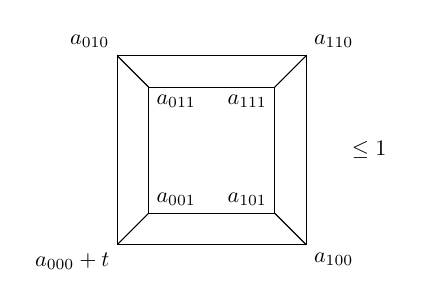
\begin{tikzpicture}[scale=0.8, every node/.style={scale=0.8}]
\draw (0,0) -- (3,0) -- (3,3) -- (0,3) -- cycle;
\draw (0.5,0.5) -- (2.5,0.5) -- (2.5,2.5) -- (0.5,2.5) -- cycle;
\draw (0,0) -- (0.5,0.5);
\draw (3,0) -- (2.5,0.5);
\draw (3,3) -- (2.5,2.5);
\draw (0,3) -- (0.5,2.5);
\node[below left] at (0,0) {$a_{000}+t$};
\node[below right] at (3,0) {$a_{100}$};
\node[above right] at (3,3) {$a_{110}$};
\node[above left] at (0,3) {$a_{010}$};

\node[above right] at (0.5,0.5) {$a_{001}$};
\node[above left] at (2.5,0.5) {$a_{101}$};
\node[below left] at (2.5,2.5) {$a_{111}$};
\node[below right] at (0.5,2.5) {$a_{011}$};

\node at (4, 1.5) {$\leq 1$};
\end{tikzpicture}
\end{center}

\end{columns}



\end{frame}